\documentclass[review]{elsarticle}

\usepackage{times}
\usepackage{graphicx}
\usepackage{amsmath,amssymb}
\usepackage{booktabs}
\usepackage{multirow}
\usepackage{xcolor}
\usepackage{caption}
\captionsetup{skip=4pt}
\usepackage[colorlinks,citecolor=blue,linkcolor=blue,urlcolor=blue]{hyperref}
\usepackage{placeins}
\renewcommand{\topfraction}{0.9}
\renewcommand{\bottomfraction}{0.8}
\renewcommand{\textfraction}{0.1}
\renewcommand{\floatpagefraction}{0.8}
\setcounter{topnumber}{4}
\setcounter{bottomnumber}{4}
\setcounter{totalnumber}{8}

\newcommand{\ms}[2]{#1{\scriptsize$\pm$#2}}

\usepackage{lineno}
\modulolinenumbers[5]

\bibliographystyle{elsarticle-num}
\begin{document}
\begin{frontmatter}

\title{IntentDiT: Prompt-Controllable Diffusion Transformer \\ for Intent-Aware Poster Layout Generation}

\author[mymainaddress]{Abdul Waheed Aagha}
\author[mymainaddress]{Seong-heum Kim\corref{mycorrespondingauthor}}
\address[mymainaddress]{School of AI Convergence, College of Information Technology, Soongsil University, Seoul, South Korea}
\cortext[mycorrespondingauthor]{Corresponding author (E-mail: seongheum@ssu.ac.kr)}

\begin{abstract}
Content-aware poster layout generation requires placing design elements without disrupting important image regions, while practical design workflows also require users to specify what should appear and where.
We propose \textbf{IntentDiT}, a prompt-controllable diffusion transformer that unifies two forms of intent: \emph{explicit} user intent, stated in a prompt, and \emph{implicit} design intent, learned from designer annotations as a placement-suitability (intent) map.
IntentDiT keeps BERT prompt tokens visible to the denoiser instead of using a single pooled sentence vector, enabling layout tokens to attend to words describing classes, counts, and spatial phrases.
When explicit positions are provided, a lightweight parser converts them into $3{\times}3$ grid position tokens that replace the learned spatial-prior keys in the same cross-attention pathway, so user instructions
override default placement during a standard diffusion sampling run, without retraining or per-prompt optimization.
We also show that standard layout metrics favor sparse generation: a frozen image-only baseline omits two or more annotated elements, which IntentDiT roughly halves.
We evaluate controllability with five template-prompt families generated from designer annotations (54K PKU and 340K CGL rows), 120 image-grounded free-form prompts per dataset with audited references, and PLA/SPLA metrics reported alongside content-aware quality metrics. IntentDiT improves audited free-form count-overlap over an external text-conditioned reference on PKU and CGL, with paired-bootstrap intervals excluding zero, and improves CGL spatial overlap.
A blinded user study further favors IntentDiT for visual quality and instruction following.

\end{abstract}

\begin{keyword}
Layout generation \sep Diffusion transformer \sep Cross-attention \sep Controllable generation \sep Content-aware poster design
\end{keyword}

\end{frontmatter}
\linenumbers

\section{Introduction}
\label{sec:intro}
Poster layout generation places design elements, including logos, headlines, body text, underlays, and decorations, on a background image. A useful model must respect image content while also following designer intent. This is harder than generic layout synthesis because element placement changes readability and
subject visibility, and because practical design workflows require user-editable control such as ``one logo at the top-left and three text boxes on the right.''

Recent diffusion and transformer models have improved layout generation quality by denoising structured element sequences~\cite{Ho20,Inoue23,Li24}.
Language interfaces have been built on top of this progress, but largely outside the continuous denoising formulation: LLM-based planners serialize layouts into discrete HTML-like token sequences or layout trees~\cite{Seol24PosterLlama,Hsu25,lin23b}, while strong image-conditioned diffusion generators such as LayoutDiT~\cite{Li24} remain image-only and cannot follow natural or semi-structured user prompts. To be specific, three gaps follow. First, prompt control has not been integrated into continuous poster-layout denoising, where content-aware conditioning and language conditioning must compete inside the same denoising step. Second, saliency maps are useful for avoiding visually prominent regions, but they are not direct models of where designers tend to place functional layout elements. Third, controllability is typically measured on blank-canvas benchmarks in which no background competes with the instruction, so prompt adherence and content preservation are rarely scored against each other.

We present \textbf{IntentDiT}, a prompt-controllable diffusion transformer for intent-aware poster layout generation.
The mechanism is intentionally lightweight: it adds no test-time optimization and no additional sampling stage. The prompt is encoded with frozen BERT and preserved as a token sequence, so the denoiser can attend to words describing element classes, counts, and spatial phrases.
If the prompt contains explicit positions, a lightweight text-spatial parser converts those phrases into position tokens on a $3{\times}3$ grid. These position tokens use the same spatial cross-attention pathway as the learned placement-suitability prior, replacing the default intent-box keys when user positions are supplied. The prompt-control mechanism therefore operates within a single standard diffusion sampling run, without retraining or per-prompt optimization: the override is a substitution of attention keys at the start of the run, not an iterative search or a separate editing stage.
For content-aware generation, IntentDiT augments image features and saliency cues with a learned placement-suitability map, adapted from density-based layout priors~\cite{Hsu23b,Hsu25}. It is an auxiliary spatial prior trained from designer annotations, and it encourages denser and more complete layouts.

\begin{figure}[!t]
  \centering
  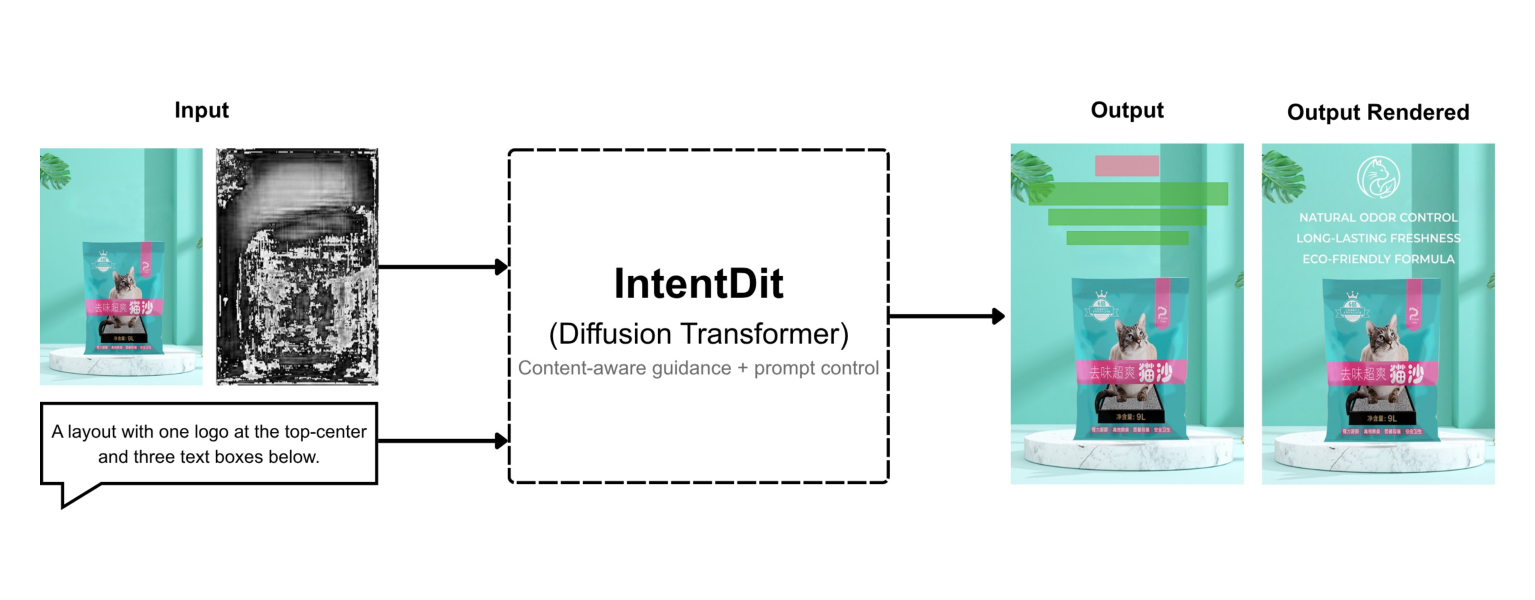
\includegraphics[width=\linewidth]{fig/fig01.pdf}
  \caption{\textbf{IntentDiT overview.} Given a background image and a structural prompt, IntentDiT generates a content-aware poster layout by combining image features, saliency cues, a learned placement-suitability map, and token-level prompt conditioning.
  }
  \label{fig:teaser}
\end{figure}

Hence, IntentDiT unifies two forms of intent within one diffusion transformer (DiT)~\cite{Peebles23}. Explicit user intent is stated in the prompt and preserved at the token level, and implicit design intent is distilled from designer annotations into the learned placement-suitability map, which we refer to as the \emph{intent map} throughout this paper. Both feed the same spatial cross-attention pathway, and when they conflict, explicit intent overrides. We accordingly call the resulting setting \emph{intent-aware} poster layout generation: content-aware generation conditioned on both forms of intent. Across two poster benchmarks, IntentDiT improves audited free-form count adherence over an external text-conditioned reference (PLA $0.694\!\rightarrow\!0.808$ on PKU and $0.614\!\rightarrow\!0.800$ on CGL, both with paired-bootstrap intervals excluding zero) and is preferred for instruction following in 91.3\% of blinded pairwise comparisons, while we report the accompanying density and structure trade-offs explicitly rather than
collapsing all metrics into a single ranking.

Our contributions are summarized as:
\begin{itemize}
  \item \textbf{Prompt-controllable diffusion transformer.}
  IntentDiT keeps prompt tokens visible to the denoiser through dense cross-attention, and uses parser-derived position tokens to override learned spatial-prior keys when explicit spatial instructions are present.
  This enables count, class, and coarse-position control within a single standard diffusion sampling run, without retraining or per-prompt optimization.

  \item \textbf{Density as a confound in layout evaluation.} We show that standard layout-quality metrics systematically favor sparse generation, and that a strong image-only baseline achieves part of its structural advantage by omitting elements, severely undercounting on 32.3\% of PKU and 50.3\% of CGL images. We therefore pair every headline comparison with count and box-area controls and paired-bootstrap intervals, and show that IntentDiT's learned placement-suitability conditioning roughly halves severe-undercount rates while participants still prefer its rendered layouts in 85.8\% of blinded quality comparisons.

  \item \textbf{Content-aware controllability evaluation.}
  We build five-family template prompt sets from designer annotations (54K PKU / 340K CGL rows), 120 image-grounded free-form prompts per dataset with single-annotator audited references and frozen manifests, and report PLA/SPLA jointly with content-aware quality metrics, paired-bootstrap intervals, and a blinded instruction-following user study.
\end{itemize}

\section{Related Work}
\label{sec:related}
\subsection{Layout generation}
Graphic layout generation has been studied with heuristic and energy-based rules~\cite{ODonovan14}, deep generative models spanning GANs and VAEs~\cite{Goodfellow14,Kingma13,Zheng19,Li19,Jyothi19}, graph- and constraint-based networks~\cite{Lee20}, and transformers~\cite{Vaswani17,Gupta21}, supported in practice by large-scale design corpora such as Rico~\cite{Deka17}. Diffusion models, first developed for image synthesis~\cite{Ho20,Ramesh21,Rombach22}, have recently advanced layout generation by iteratively denoising a structured layout representation~\cite{Inoue23,Li23RADM}.

Poster-specific work targets the content-aware setting used in this paper. For example, CGL-GAN~\cite{Zhou22} and DS-GAN~\cite{Hsu23a} introduce the CGL and PKU benchmarks together with composition-aware generators. ICVT aligns geometry in an image-conditioned variational transformer~\cite{Cao22}. RALF augments generation with retrieved neighbor layouts~\cite{Horita24}. LayoutDiT balances background content and layout structure with a diffusion transformer~\cite{Li24}, and UniLayDiff unifies several constraint-conditioned layout tasks in a diffusion-transformer framework~\cite{Liu25UniLayDiff}. These methods provide strong image-conditioned baselines but are not designed around direct prompt control in continuous poster-layout denoising. %with a learned placement-suitability prior.

\subsection{Text-guided and controllable layouts}
Language and high-level constraints such as element counts, spatial relations, and hierarchy offer an intuitive interface for specifying layouts. Prior work studied conditional generation and controllability for graphics and layouts~\cite{Li19,Jyothi19,Gupta21}. More recent approaches explore text-to-layout generation and constraint following via autoregressive transformers or large language models. LayoutFormer++ serializes constraints for conditional decoding~\cite{Jiang23}, and Parse-Then-Place separates textual parsing from placement~\cite{lin23a}. These works are evaluated on blank-canvas benchmarks (e.g., Rico~\cite{Deka17}, PubLayNet~\cite{Zhong19}) without a conditioning background image. LayoutPrompter~\cite{lin23b} generates layouts from serialized textual descriptions via in-context LLM prompting. It additionally addresses content-aware generation, but plans in a discrete token space rather than denoising a continuous layout.

In the content-aware poster domain, RADM couples diffusion with visual-textual and geometry relation
modules~\cite{Li23RADM}. PosterLlama reformats layouts as HTML-like token sequences for LLM decoding~\cite{Seol24PosterLlama}. PosterO structures layout trees to enable LLM-based generalized content-aware generation~\cite{Hsu25} and inspires the external text-conditioned reference used in our evaluation protocol. PosterLLaVa and POSTA build multimodal-LLM design pipelines~\cite{Yang24,Chen25}, and iPoster applies graph-enhanced diffusion under user-specified constraints~\cite{Zhou26iPoster}.

Our work differs from these systems in three respects. First, LLM-based planners operate in a discrete HTML- or sequence-token space, whereas we apply prompt control inside continuous layout denoising. Second, RADM conditions on the textual content to be rendered on the poster, whereas our prompts are structural instructions about element counts, classes, and coarse positions. Third, iPoster expresses user constraints as graphs, whereas our system accepts free-form natural language and resolves explicit spatial phrases through a parser-driven override of attention keys. We integrate token-level text conditioning (dense cross-attention) into a continuous diffusion transformer backbone for content-aware poster layout generation, and couple it with a learned density-based placement-suitability prior.

\subsection{Spatial priors beyond saliency}
Saliency maps highlight visually prominent regions and are often useful as avoidance cues, but they do not directly encode layout utility. They are not designed to represent layout utility where designers tend to place elements.
A complementary line of work models this positive signal directly. DensityLayout~\cite{Hsu23b} introduces density-conditioned layout generation, and shows that density-based design priors can encode where layout elements tend to appear. PosterO~\cite{Hsu25} structures layout trees with design-aware priors. Our IntentDiT adapts this idea into a learned placement-suitability map, referred to as the intent map in this paper, used as auxiliary conditioning in a diffusion transformer. The map is a learned spatial prior, not direct evidence of human semantic intent, and not universally superior to all simple priors.

\section{Proposed Method}
\label{sec:method}

\subsection{Problem Setup and Diffusion Backbone}
\label{sec:problem}

Given a background image $I$ and optional text prompt $T$, we generate a layout
$\mathcal{L}=\{(b_i,c_i)\}_{i=1}^{N}$, where $b_i=(x_i,y_i,w_i,h_i)\in[0,1]^4$ is a normalized box and $c_i$ is an element class.
Following LayoutDiT~\cite{Li24}, each element is represented as a token containing a class vector and box coordinates.
The forward diffusion process corrupts a clean layout $\mathbf{L}_0$:
\begin{equation}
q(\mathbf{L}_t|\mathbf{L}_0)=
\mathcal{N}(\mathbf{L}_t;\sqrt{\bar{\alpha}_t}\mathbf{L}_0,(1-\bar{\alpha}_t)\mathbf{I}),
\end{equation}
and a transformer denoiser $\epsilon_\theta$ predicts the noise.
All reported IntentDiT inference uses a cosine DDIM sampler with 100 steps, matching the cosine training schedule.

\subsection{Prompt-Controllable Conditioning}
\label{sec:prompt_conditioning}

IntentDiT uses two prompt pathways.
First, a frozen BERT-base encoder~\cite{Devlin19} produces token-level embeddings
\begin{equation}
\mathbf{H}_{\text{text}}\in\mathbb{R}^{L\times d_{\text{text}}},
\end{equation}
which are projected to the diffusion-transformer dimension and used as keys/values in text-token cross-attention.
This avoids compressing the prompt into a single pooled vector: each layout token can attend directly to the full sequence of prompt tokens, preserving class, count, and spatial information.
Cross-attention enables this routing, but it does not guarantee that every element always attends to the semantically correct word; Sec.~\ref{sec:ablation_note} reports the pooled-embedding ablation that supports this design choice.

Second, when a prompt contains explicit spatial phrases, a lightweight text-spatial parser extracts class and position assignments on a $3{\times}3$ grid.
Each assignment is encoded as a class one-hot vector plus a normalized grid-region box and projected by an MLP.
During denoising, these text-spatial tokens replace the learned intent-box keys in the shared spatial cross-attention pathway.
The user instruction therefore overrides the model's default placement prior in the same architecture, without retraining, sampling-time optimization, or a separate editing stage.

\subsection{Placement-Suitability Map and Spatial Priors}
\label{sec:intent_map}

For content awareness, IntentDiT conditions on image features, saliency, and a learned placement-suitability map.
The saliency map provides a negative cue: important visual regions should often remain uncovered.
The learned map provides a positive cue: regions where designers tend to place layout elements.
We train a U-Net with a MiT-B1 encoder~\cite{Ronneberger15} to regress density masks rasterized from train-split layout boxes.
Separate PKU and CGL predictors are trained on official training splits only.
We use the final checkpoints from archived 100-epoch PKU and 35-epoch CGL predictor training runs; they were frozen before layout-generator evaluation, and no layout-generator validation or test metric was used for selection.
Test maps are generated from background/inpaint images only and do not read test boxes.

\subsection{IntentDiT Architecture}
\label{sec:architecture}

\begin{figure*}[!t]
  \centering
  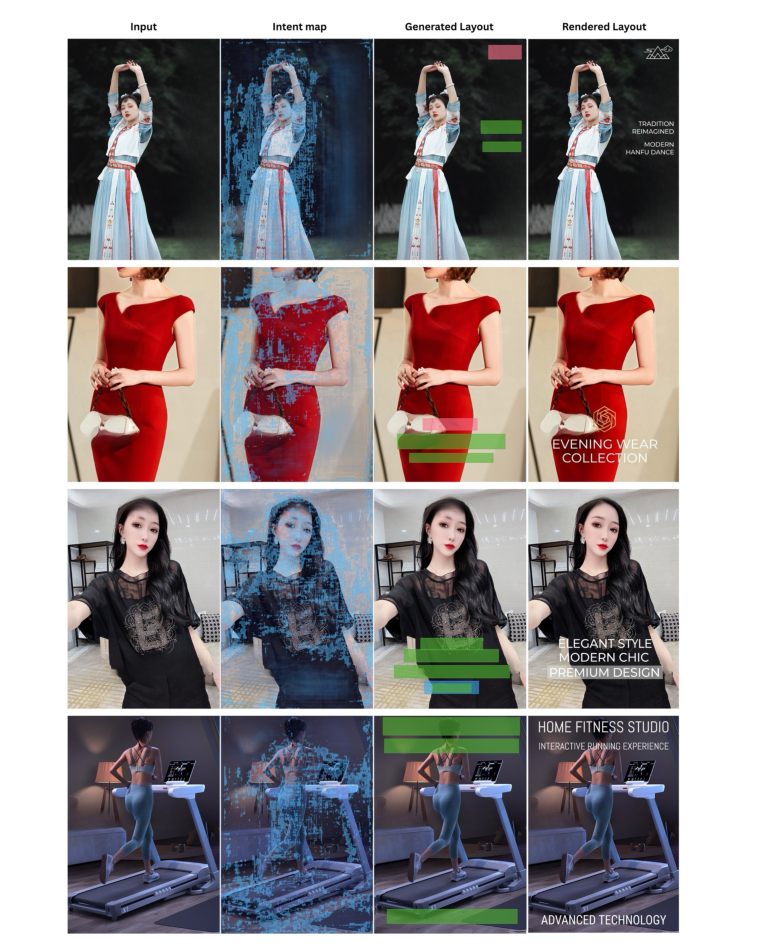
\includegraphics[width=\textwidth]{fig/fig02.pdf}
  \caption{\textbf{IntentDiT architecture.}
  Image, saliency, placement-suitability, and prompt features condition the layout denoiser through self- and cross-attention. When a prompt specifies explicit locations, parsed 3×3 position tokens replace the placement-suitability tokens in the shared spatial-conditioning pathway.}
  \label{fig:architecture}
\end{figure*}

Figure~\ref{fig:architecture} summarizes the model.
The RGB image and selected saliency/intent maps are concatenated as visual channels and encoded by a ViT-style or Swin-style backbone.
Dominant saliency and intent regions are also converted into bounding boxes and encoded by MLPs, giving the decoder compact geometric keys.
A query-based module predicts a positive content-guidance weight $w_{\mathrm{CGB}}$ that scales image cross-attention.
Each denoising block applies: layout self-attention, image cross-attention, saliency-box cross-attention, intent-box or text-spatial cross-attention, text-token cross-attention, and a feed-forward network.

\subsection{Training Objective}
\label{sec:objective}

We train with denoising, count-alignment, and placement losses:
\begin{equation}
\mathcal{L}_{\text{total}}=
\mathcal{L}_{\text{denoise}}+\lambda_1\mathcal{L}_{\text{text}}+\lambda_2\mathcal{L}_{\text{intent}}.
\end{equation}
$\mathcal{L}_{\text{denoise}}$ is standard diffusion noise prediction.
$\mathcal{L}_{\text{text}}$ aligns predicted and requested per-class counts.
Implementation-wise, predicted counts are differentiable expected counts obtained by summing softmax probabilities over non-padding classes across layout tokens; the null/padding class is excluded.
The placement loss assigns each valid predicted element to its best valid intent region:
\begin{equation}
\mathcal{L}_{\text{intent}}=
1-\frac{1}{N_v}\sum_{i\in\mathcal{V}}\max_{j\in\mathcal{I}}
\operatorname{IoU}(\hat b_i,b^{\text{intent}}_j).
\end{equation}
Intent-box padding is encoded as $-1$ and masked, so padded regions do not affect the objective.
We use $\lambda_1=0.1$ and $\lambda_2=0.05$ by default.

\subsection{Implementation Details}
\label{sec:implementation_details}

The layout denoiser uses hidden dimension 512 with eight attention heads, two transformer encoder layers, and four decoder layers.
The visual backbone is a jointly trained ViT-style or shifted-window encoder with $32{\times}32$ patches, six visual encoder blocks, and $384{\times}256$ input resolution; the main reported model uses the ViT-style encoder.
Layouts are padded to a maximum of 16 elements with a null class token.
The frozen BERT-base text encoder uses a maximum prompt length of 128 tokens, and text-conditioned training samples a random prompt variant per image per epoch from the five-family prompt mixture.
PKU models are trained with batch size 32 and learning rate $10^{-4}$; CGL models use batch size 128 and learning rate $2{\times}10^{-4}$.
All layout generators are trained for 500 epochs with Adam, cosine learning-rate annealing, gradient clipping at 1.0, and three independent training seeds for the primary variants.
Reported checkpoints are fixed a priori to the final 500-epoch checkpoint; validation monitoring is diagnostic only and is not used for test-set model selection.
At inference, generated boxes are clamped to $[0,1]$ and degenerate boxes are filtered before evaluation.

\section{Results and Discussion}
\label{sec:experiments}

\subsection{Setup}
\label{sec:setup}

\textbf{Datasets.}
We evaluate on PKU PosterLayout~\cite{Hsu23a} and CGL~\cite{Zhou22} using official train/validation/test splits.
PKU contains 7,734/1,000/1,000 train/validation/test posters, and CGL contains 48,544/6,002/6,002.
Models are trained for 500 epochs with three seeds for primary variants.

\textbf{Prompt data.}
From train annotations, we generate five prompt families:
Basic count prompts, Enhanced count+coarse-position prompts, Advanced distribution prompts, Spatial per-element $3{\times}3$ prompts, and Rich paraphrased/synonym prompts.
This yields 54,138 PKU and 339,808 CGL training prompt rows.
For harder evaluation, we add 120 image-grounded free-form prompts per dataset.
Free-form prompts are manually audited using a single-annotator prompt-level reference.
Ambiguous/out-of-schema rows are excluded from parser-accuracy denominators, but fixed manual interpretations are retained for all-120 coverage metrics.

\textbf{Baselines and protocol.}
For image-only evaluation, we use frozen LayoutDiT reference tensors for the LayoutDiT baseline~\cite{Li24}.
The exact sampler configuration used to produce these tensors was not preserved.
The comparison standardizes the dataset split, tensor format, and evaluator, but is not a same-sampler ablation.
For free-form text evaluation, we use a standardized external text-conditioned reference tensor derived from an external layout-tree/text-conditioned pipeline inspired by PosterO~\cite{Hsu25}; we do not claim an official PosterO reproduction.

\textbf{Metrics.}
We report standard content-aware layout metrics from prior work~\cite{Li24}: Val, OOB, Ove, Uti, Occ, Rea, UndS, paired IoU, MaxIoU, and Type-F1.
Val is the non-degenerate-element validity score: one minus the fraction of predicted non-padding elements whose clamped box area is below $10^{-3}$.
We also report Prompt-Layout Alignment (PLA) and spatial PLA (SPLA).
For prompt counts $n_k^{\text{prompt}}$ and generated counts $n_k^{\text{gen}}$, PLA is
\begin{equation}
\text{PLA}=1-\frac{\sum_k |n_k^{\text{gen}}-n_k^{\text{prompt}}|}
{\sum_k(n_k^{\text{gen}}+n_k^{\text{prompt}})}.
\end{equation}
If a prompt requests zero elements but the model generates a nonempty layout, PLA is 0.
SPLA scores spatial-phrase adherence rather than count/type adherence.
Let $\mathcal{G}_k^{\text{prompt}}$ be the multiset of $3{\times}3$ grid cells requested for class $k$ and $\mathcal{G}_k^{\text{gen}}$ the multiset of cells occupied by the snapped centers of generated class-$k$ elements; SPLA is the request-weighted fraction of requested positions that are matched:
\begin{equation}
\text{SPLA}=\frac{\sum_{k}\bigl|\mathcal{G}_k^{\text{gen}}\cap\mathcal{G}_k^{\text{prompt}}\bigr|}{\sum_{k}\bigl|\mathcal{G}_k^{\text{prompt}}\bigr|},
\end{equation}
where $\cap$ is multiset intersection (each requested cell is matched at most once) and prompts with no spatial phrases are excluded.
A layout with correct counts but displaced elements therefore scores below one on SPLA even though it scores well on PLA.
We report diagnostic HFD as a Fr\'echet distance over handcrafted count/geometry features, not official LayoutFID.

\subsection{Image-Only Content-Aware Generation}
\label{sec:image_results}

Tables~\ref{tab:image_quality} and~\ref{tab:density_controls_compact} summarize the image-only comparison with frozen LayoutDiT reference tensors.
IntentDiT generates denser layouts with higher utilization on both datasets and a significant CGL Type-F1 gain.
The same density shift introduces structural trade-offs: LayoutDiT has lower OOB/Ove/Occ and higher MaxIoU/UndS.
We therefore do not claim uniform image-only superiority; the evidence supports a trade-off between density and structure.

\begin{table}[!t]
\caption{\textbf{Image-only comparison with shared evaluator.}
IntentDiT uses ViT+Saliency+Intent and reports mean$\pm$std over three seeds.
LayoutDiT is a frozen reference tensor.}
\label{tab:image_quality}
\centering
\scriptsize
\setlength{\tabcolsep}{3pt}
\resizebox{\linewidth}{!}{%
\begin{tabular}{llccccccc}
\toprule
\textbf{Dataset} & \textbf{Method} & OOB$\downarrow$ & Ove$\downarrow$ & Uti$\uparrow$ & Occ$\downarrow$ & UndS$\uparrow$ & MaxIoU$\uparrow$ & Type-F1$\uparrow$ \\
\midrule
PKU & LayoutDiT & \textbf{0.014} & \textbf{0.003} & 0.179 & \textbf{0.120} & \textbf{0.956} & \textbf{0.506} & 0.717 \\
PKU & \textbf{IntentDiT} & \ms{0.031}{.006} & \ms{0.041}{.003} & \textbf{\ms{0.287}{.006}} & \ms{0.157}{.001} & \ms{0.711}{.052} & \ms{0.366}{.008} & \textbf{\ms{0.725}{.001}} \\
\midrule
CGL & LayoutDiT & \textbf{0.006} & \textbf{0.002} & 0.162 & \textbf{0.116} & \textbf{0.977} & \textbf{0.660} & 0.680 \\
CGL & \textbf{IntentDiT} & \ms{0.043}{.003} & \ms{0.053}{.002} & \textbf{\ms{0.298}{.001}} & \ms{0.158}{.003} & \ms{0.642}{.016} & \ms{0.383}{.005} & \textbf{\ms{0.705}{.002}} \\
\bottomrule
\end{tabular}
}
\end{table}

\begin{table}[!t]
\caption{\textbf{Density controls for image-only comparison.}
Count error is $n_{\text{pred}}-n_{\text{gt}}$.
Severe undercount means at least two fewer predicted elements than ground truth.}
\label{tab:density_controls_compact}
\centering
\scriptsize
\setlength{\tabcolsep}{4pt}
\begin{tabular}{llccccc}
\toprule
\textbf{Dataset} & \textbf{Method} & $n_{\text{pred}}$ & Count err. & Severe under$\downarrow$ & Total area & Mean area \\
\midrule
PKU & LayoutDiT & 3.699 & -0.704 & 0.323 & 0.147 & 0.040 \\
PKU & \textbf{IntentDiT} & \textbf{\ms{4.865}{.110}} & \textbf{\ms{0.462}{.110}} & \textbf{\ms{0.177}{.012}} & \textbf{\ms{0.316}{.011}} & \textbf{\ms{0.065}{.001}} \\
\midrule
CGL & LayoutDiT & 3.250 & -1.625 & 0.503 & 0.123 & 0.038 \\
CGL & \textbf{IntentDiT} & \textbf{\ms{5.368}{.066}} & \textbf{\ms{0.493}{.066}} & \textbf{\ms{0.224}{.007}} & \textbf{\ms{0.346}{.004}} & \textbf{\ms{0.064}{.000}} \\
\bottomrule
\end{tabular}
\end{table}

\begin{table}[!t]
\caption{\textbf{Paired bootstrap summary for headline image-only comparison.}
Positive oriented deltas favor IntentDiT; for lower-is-better metrics, delta is LayoutDiT minus IntentDiT.}
\label{tab:bootstrap_compact}
\centering
\scriptsize
\begin{tabular}{llcc}
\toprule
\textbf{Dataset} & \textbf{Metric} & \textbf{Delta} & \textbf{95\% CI} \\
\midrule
PKU & Occ & -0.0360 & [-0.0439, -0.0279] \\
PKU & MaxIoU & -0.1403 & [-0.1573, -0.1248] \\
PKU & Type-F1 & +0.0087 & [-0.0043, 0.0218] \\
\midrule
CGL & Occ & -0.0420 & [-0.0469, -0.0367] \\
CGL & MaxIoU & -0.2750 & [-0.2831, -0.2670] \\
CGL & Type-F1 & +0.0245 & [0.0183, 0.0309] \\
\bottomrule
\end{tabular}
\end{table}

\subsection{Prompt-Based Controllability}
\label{sec:control}

\begin{figure}[!t]
  \centering
  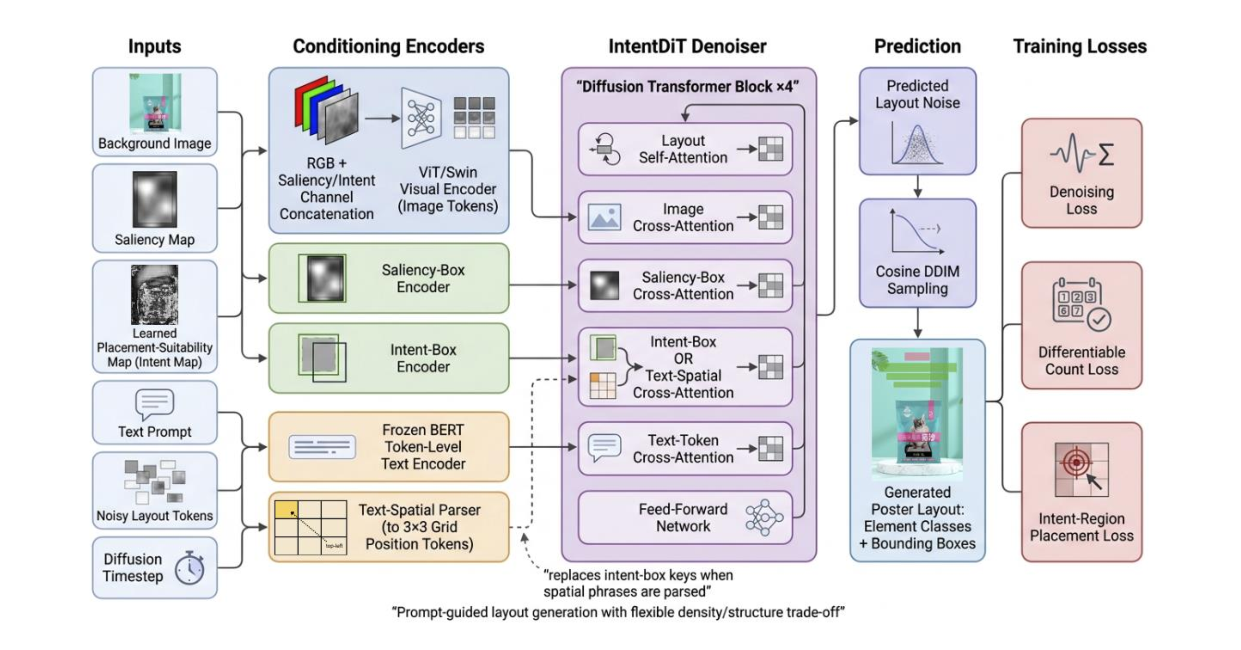
\includegraphics[width=\linewidth]{fig/fig03.pdf}
  \caption{\textbf{Qualitative prompt-control examples.} Each column shows, from top to bottom, the rendered poster layout, predicted bounding boxes, and input background image; the corresponding prompt is shown below. The examples illustrate control over element classes, counts, underlays, and coarse spatial positions.}
  \label{fig:prompt_editing}
\end{figure}

Table~\ref{tab:freeform} evaluates 120 free-form prompts per dataset using manually audited references.
IntentDiT improves count-overlap and exact-count match on both datasets, and improves CGL spatial overlap.
Paired-bootstrap 95\% intervals confirm these PLA and exact-count gains are reliable on both datasets, along with the CGL SPLA gain (Table~\ref{tab:bootstrap_freeform}), so the controllability improvement is not an artifact of a single evaluation split.
The parser that powers the positional-override mechanism (Sec.~\ref{sec:prompt_conditioning}) was manually audited against all 120 free-form prompts per dataset and found accurate on the large majority of position assignments (position F1 0.953 on PKU, 0.943 on CGL), so the remaining free-form gap is concentrated in spatial grounding under natural phrasing rather than in parser activation itself.
The result is nevertheless not a solved natural-language layout-control result: PKU structural metrics and Type-F1 favor the external text reference, and CGL still shows a Type-F1 trade-off.
This is why prompt adherence is reported together with content-aware quality metrics.

\begin{table}[!t]
\caption{\textbf{Paired bootstrap summary for the free-form controllability comparison.}
Positive deltas favor IntentDiT over the external text reference. Intervals are 95\% paired seed$\times$image bootstrap intervals over the all-120 manual reference.}
\label{tab:bootstrap_freeform}
\centering
\scriptsize
\begin{tabular}{llcc}
\toprule
\textbf{Dataset} & \textbf{Metric} & \textbf{Delta} & \textbf{95\% CI} \\
\midrule
PKU & ExactCount & +0.1639 & [0.0750, 0.2528] \\
PKU & PLA & +0.1137 & [0.0732, 0.1547] \\
PKU & SPLA & +0.0147 & [-0.0227, 0.0512] \\
\midrule
CGL & ExactCount & +0.1639 & [0.0833, 0.2500] \\
CGL & PLA & +0.1866 & [0.1504, 0.2241] \\
CGL & SPLA & +0.1663 & [0.1152, 0.2199] \\
\bottomrule
\end{tabular}
\end{table}

\begin{table}[!t]
\caption{\textbf{Free-form prompt comparison on 120-image subsets.}
Prompt-adherence metrics use manually audited references.
IntentDiT is mean$\pm$std over three seeds; the external text-conditioned reference is a single frozen tensor.}
\label{tab:freeform}
\centering
\scriptsize
\setlength{\tabcolsep}{3pt}
\resizebox{\linewidth}{!}{%
\begin{tabular}{llccccccccc}
\toprule
\textbf{Dataset} & \textbf{Method} & Val$\uparrow$ & OOB$\downarrow$ & Occ$\downarrow$ & Rea$\downarrow$ & Exact$\uparrow$ & PLA$\uparrow$ & SPLA$\uparrow$ & Type-F1$\uparrow$ & HFD$\downarrow$ \\
\midrule
PKU & External text reference & 0.991 & \textbf{0.023} & \textbf{0.141} & \textbf{0.010} & 0.083 & 0.694 & 0.256 & \textbf{0.756} & \textbf{0.031} \\
PKU & \textbf{IntentDiT} & \textbf{\ms{0.997}{.000}} & \ms{0.073}{.017} & \ms{0.161}{.005} & \ms{0.014}{.000} & \textbf{\ms{0.247}{.037}} & \textbf{\ms{0.808}{.018}} & \textbf{\ms{0.271}{.006}} & \ms{0.658}{.033} & \ms{0.232}{.042} \\
\midrule
CGL & External text reference & \textbf{0.991} & 0.049 & 0.215 & 0.016 & 0.025 & 0.614 & 0.183 & \textbf{0.662} & \textbf{0.117} \\
CGL & \textbf{IntentDiT} & \ms{0.987}{.008} & \textbf{\ms{0.043}{.009}} & \textbf{\ms{0.149}{.008}} & \textbf{\ms{0.016}{.001}} & \textbf{\ms{0.189}{.045}} & \textbf{\ms{0.800}{.010}} & \textbf{\ms{0.349}{.019}} & \ms{0.641}{.012} & \ms{0.375}{.033} \\
\bottomrule
\end{tabular}
}
\end{table}

\begin{table}[!t]
\caption{\textbf{Free-form density controls.}
Manual request counts are used for all 120 prompts.
Occ$_{\text{match}}$/Rea$_{\text{match}}$ are descriptive because exact-count-matched subsets are small.}
\label{tab:freeform_density}
\centering
\scriptsize
\setlength{\tabcolsep}{3pt}
\resizebox{\linewidth}{!}{%
\begin{tabular}{llccccccccc}
\toprule
\textbf{Dataset} & \textbf{Method} & $n_{\text{req}}$ & $n_{\text{pred}}$ & Count err. & Small$\downarrow$ & Severe under$\downarrow$ & Total area & Mean area & Occ$_{\text{match}}\downarrow$ & Rea$_{\text{match}}\downarrow$ \\
\midrule
PKU & External text reference & 3.608 & 4.408 & 0.800 & 0.013 & 0.067 & 0.176 & 0.050 & 0.081 & 0.015 \\
PKU & \textbf{IntentDiT} & \ms{3.608}{.000} & \ms{3.433}{.067} & \ms{-0.175}{.067} & \ms{0.006}{.003} & \ms{0.072}{.017} & \ms{0.190}{.002} & \ms{0.056}{.001} & \ms{0.102}{.035} & \ms{0.012}{.002} \\
\midrule
CGL & External text reference & 3.592 & 4.050 & 0.458 & 0.034 & 0.150 & 0.208 & 0.071 & 0.250 & 0.016 \\
CGL & \textbf{IntentDiT} & \ms{3.592}{.000} & \ms{3.678}{.180} & \ms{0.086}{.180} & \ms{0.030}{.002} & \ms{0.067}{.012} & \ms{0.175}{.016} & \ms{0.048}{.002} & \ms{0.158}{.028} & \ms{0.016}{.002} \\
\bottomrule
\end{tabular}
}
\end{table}

\subsection{Ablation Study}
\label{sec:ablation_note}

The focused ablations in Table~\ref{tab:ablation_compact} support two design choices.
First, token-level text conditioning improves Basic-prompt PLA and Type-F1 compared with pooled sentence conditioning.
Second, among the tested image-only variants, Saliency+Intent gives the lowest Occ and Rea, while Saliency alone gives higher UndS.

\begin{table}[!t]
\caption{\textbf{Compact ablations on PKU.}
Rows are mean$\pm$std over three seeds.
The first block changes only the text-conditioning interface; the second block reports selected conditioning variants.}
\label{tab:ablation_compact}
\centering
\scriptsize
\setlength{\tabcolsep}{3pt}
\resizebox{\linewidth}{!}{%
\begin{tabular}{llccccc}
\toprule
\textbf{Protocol} & \textbf{Variant} & PLA$\uparrow$ & Type-F1$\uparrow$ & Occ$\downarrow$ & Rea$\downarrow$ & UndS$\uparrow$ \\
\midrule
Text mode & Pooled sentence & \ms{0.808}{.003} & \ms{0.866}{.005} & \ms{0.164}{.002} & \ms{0.015}{.000} & \ms{0.348}{.021} \\
Text mode & Token-level cross-attention & \textbf{\ms{0.839}{.001}} & \textbf{\ms{0.961}{.005}} & \textbf{\ms{0.161}{.001}} & \ms{0.015}{.000} & \textbf{\ms{0.401}{.010}} \\
\midrule
Image-only & Saliency & N/A & N/A & \ms{0.165}{.002} & \ms{0.015}{.001} & \textbf{\ms{0.744}{.027}} \\
Image-only & Intent & N/A & N/A & \ms{0.192}{.001} & \ms{0.016}{.000} & \ms{0.736}{.052} \\
Image-only & Saliency+Intent & N/A & N/A & \textbf{\ms{0.157}{.001}} & \textbf{\ms{0.014}{.000}} & \ms{0.711}{.052} \\
\bottomrule
\end{tabular}
}
\end{table}

\subsection{User Study}
\label{sec:user_study}

We also conducted a blinded web-based user study with 30 participants.
Part~A compared IntentDiT with LayoutDiT for visual quality and with the external text reference for instruction following; ties were allowed and excluded from the win-rate denominator.
Part~B rated common failure severity on a seven-point scale.
The study uses frozen rendered stimuli and randomized left/right ordering, and complements rather than replaces automatic evaluation.
Participants preferred IntentDiT in 85.8\% of non-tie visual-quality comparisons and 91.3\% of instruction-following comparisons (Table~\ref{tab:user_study_compact}).

\begin{table}[!t]
\caption{\textbf{User-study summary.}
Confidence intervals are descriptive bootstrap intervals over participants/items.}
\label{tab:user_study_compact}
\centering
\small
\resizebox{\linewidth}{!}{%
\begin{tabular}{llccc}
\toprule
\textbf{Part} & \textbf{Comparison / rating} & \textbf{Participants} & \textbf{N} & \textbf{Result} \\
\midrule
A & Quality vs.\ LayoutDiT & 30 & 798 non-ties & 85.8\% preference [76.5, 93.3] \\
A & Instruction vs.\ external text reference & 30 & 837 non-ties & 91.3\% preference [86.3, 95.6] \\
\midrule
B & Subject occlusion severity & 30 & 150 ratings & 5.97 mean / 6 median \\
B & Illegible text severity & 30 & 150 ratings & 5.87 mean / 6 median \\
B & Element overlap severity & 30 & 150 ratings & 4.73 mean / 5 median \\
B & Count mismatch severity & 30 & 150 ratings & 4.16 mean / 4 median \\
\bottomrule
\end{tabular}
}
\end{table}

\subsection{Limitations}
\label{sec:limitations}

Several limitations remain.
Free-form spatial grounding is still substantially harder than canonical template prompts, and exact count satisfaction remains modest in absolute terms.
Layout-quality metrics are density-sensitive: denser predictions improve completeness and utilization but can worsen OOB, overlap, occlusion, and MaxIoU.
The learned placement-suitability map is an auxiliary prior; diagnostics compare it with simple maps, but we have not retrained every simple prior inside the generator.
The user study is blinded and participant-aware, but it includes 30 design-aware participants rather than a large crowd panel.
Finally, HFD is a diagnostic handcrafted feature distance and should not be interpreted as official LayoutFID.

\section{Conclusion}
\label{sec:conclusion}

We introduced IntentDiT, a prompt-controllable diffusion transformer for content-aware poster layout generation.
The method keeps prompt tokens visible to the denoiser, converts explicit spatial phrases into position tokens that override the learned spatial-prior pathway, and uses a learned placement-suitability map as auxiliary content-aware conditioning.
The results support a narrower but stronger claim: IntentDiT improves prompt adherence and produces denser, more complete layouts, while preserving transparent reporting of density and structure trade-offs against strong frozen baselines.
This makes it a practical step toward user-controllable poster layout generation, while leaving open future work on stronger free-form spatial grounding, official distributional metrics, and generator-level comparisons to simple spatial priors.

\section*{Acknowledgements}
This research was supported by G-LAMP Program of the National Research Foundation of Korea (NRF) grant funded by the Ministry of Education
(No.~RS-2025-25441317). This work was also supported by the NRF grant funded by the Ministry of Science and ICT (MSIT) (RS-2025-16071992), and by MSIT and the National IT Industry Promotion Agency through the Advanced GPU Utilization Support Program (02-26-01-0499). \\
The authors thank the user-study participants for their time and feedback.

\section*{Ethics statement}
The user study involved adult volunteers.
Participants were informed of the study's purpose, participated anonymously through a web interface, provided informed consent before participation, and could withdraw at any time.
No personally identifying information was collected, and only publicly released benchmark images from PKU PosterLayout and CGL were shown.

\section*{Code availability}
Source code and reproducibility scripts are available at \url{https://github.com/aaghakr/layoutdit}.





\FloatBarrier
\bibliography{layoutgen}

\end{document}
